% Generated by eval/scripts/write_uriel_latex_assets.py. Do not edit by hand.
\definecolor{UrielRomance}{HTML}{D55E00}
\definecolor{UrielGermanic}{HTML}{0072B2}
\definecolor{UrielUralic}{HTML}{009E73}
\definecolor{UrielSlavic}{HTML}{6A51A3}
\definecolor{UrielSemitic}{HTML}{E69F00}
\definecolor{UrielBantu}{HTML}{5A8F29}
\definecolor{UrielClose}{HTML}{355C7D}
\definecolor{UrielMiddle}{HTML}{4ECDC4}
\definecolor{UrielFar}{HTML}{F0932B}
\definecolor{SpeakerTiny}{HTML}{88CCEE}
\definecolor{SpeakerSmall}{HTML}{44AA99}
\definecolor{SpeakerMedium}{HTML}{DDCC77}
\definecolor{SpeakerLarge}{HTML}{CC6677}
\definecolor{SpeakerHuge}{HTML}{882255}

\newcommand{\UrielDistanceMatrixTable}{%
\begin{landscape}
\begin{table}[p]
\centering
\caption[URIEL+ featural distance matrix]{URIEL+ featural angular distance matrix for the selected attack languages. Lower values indicate closer languages; higher values indicate greater typological distance.}
\label{tab:urielplus-distances}
\begingroup
\scriptsize
\setlength{\tabcolsep}{3.2pt}
\renewcommand{\arraystretch}{1.18}
\begin{adjustbox}{width=0.9\linewidth,center}
\begin{tabular}{>{\raggedright\arraybackslash}p{2.85cm}|*{13}{>{\centering\arraybackslash}p{0.88cm}}}
\hline
\textbf{Language} & \cellcolor[HTML]{F7D7CF}\textbf{\texttt{ita}} & \cellcolor[HTML]{F7D7CF}\textbf{\texttt{por}} & \cellcolor[HTML]{F7D7CF}\textbf{\texttt{spa}} & \cellcolor[HTML]{D6E6F6}\textbf{\texttt{eng}} & \cellcolor[HTML]{D6E6F6}\textbf{\texttt{dan}} & \cellcolor[HTML]{D6E6F6}\textbf{\texttt{nor}} & \cellcolor[HTML]{D6E6F6}\textbf{\texttt{swe}} & \cellcolor[HTML]{D8F0E1}\textbf{\texttt{fin}} & \cellcolor[HTML]{E8DDF5}\textbf{\texttt{bul}} & \cellcolor[HTML]{E8DDF5}\textbf{\texttt{rus}} & \cellcolor[HTML]{E8DDF5}\textbf{\texttt{ukr}} & \cellcolor[HTML]{F8E2C2}\textbf{\texttt{ara}} & \cellcolor[HTML]{DCEBC8}\textbf{\texttt{swa}} \\
\hline
\cellcolor[HTML]{F7D7CF}\textbf{\mbox{Italian (\texttt{ita})}} & \cellcolor[HTML]{E6E6E6}\textemdash & \cellcolor[HTML]{3F8899}\textcolor{black}{0.316} & \cellcolor[HTML]{49B7B6}\textcolor{black}{0.418} & \cellcolor[HTML]{58CEC1}\textcolor{black}{0.476} & \cellcolor[HTML]{99D8AB}\textcolor{black}{0.533} & \cellcolor[HTML]{D6E097}\textcolor{black}{0.586} & \cellcolor[HTML]{80D4B4}\textcolor{black}{0.510} & \cellcolor[HTML]{6ED2BA}\textcolor{black}{0.494} & \cellcolor[HTML]{4CC4BE}\textcolor{black}{0.446} & \cellcolor[HTML]{50CDC3}\textcolor{black}{0.469} & \cellcolor[HTML]{48B3B4}\textcolor{black}{0.410} & \cellcolor[HTML]{9DD8AA}\textcolor{black}{0.536} & \cellcolor[HTML]{85D5B2}\textcolor{black}{0.515} \\
\cellcolor[HTML]{F7D7CF}\textbf{\mbox{Portuguese (\texttt{por})}} & \cellcolor[HTML]{3F8899}\textcolor{black}{0.316} & \cellcolor[HTML]{E6E6E6}\textemdash & \cellcolor[HTML]{46AAAE}\textcolor{black}{0.391} & \cellcolor[HTML]{48B3B3}\textcolor{black}{0.409} & \cellcolor[HTML]{72D2B8}\textcolor{black}{0.498} & \cellcolor[HTML]{9BD8AB}\textcolor{black}{0.534} & \cellcolor[HTML]{4ECCC4}\textcolor{black}{0.465} & \cellcolor[HTML]{4BC2BD}\textcolor{black}{0.442} & \cellcolor[HTML]{45A3AA}\textcolor{black}{0.375} & \cellcolor[HTML]{4CC5BF}\textcolor{black}{0.450} & \cellcolor[HTML]{47AEB1}\textcolor{black}{0.400} & \cellcolor[HTML]{79D3B6}\textcolor{black}{0.505} & \cellcolor[HTML]{60D0BE}\textcolor{black}{0.483} \\
\cellcolor[HTML]{F7D7CF}\textbf{\mbox{Spanish (\texttt{spa})}} & \cellcolor[HTML]{49B7B6}\textcolor{black}{0.418} & \cellcolor[HTML]{46AAAE}\textcolor{black}{0.391} & \cellcolor[HTML]{E6E6E6}\textemdash & \cellcolor[HTML]{4ECDC4}\textcolor{black}{0.466} & \cellcolor[HTML]{4ABAB8}\textcolor{black}{0.426} & \cellcolor[HTML]{BFDD9F}\textcolor{black}{0.566} & \cellcolor[HTML]{A2D9A8}\textcolor{black}{0.541} & \cellcolor[HTML]{6AD1BB}\textcolor{black}{0.491} & \cellcolor[HTML]{4DC9C1}\textcolor{black}{0.457} & \cellcolor[HTML]{4CC5BF}\textcolor{black}{0.450} & \cellcolor[HTML]{56CEC1}\textcolor{black}{0.473} & \cellcolor[HTML]{77D3B6}\textcolor{black}{0.503} & \cellcolor[HTML]{75D3B7}\textcolor{black}{0.501} \\
\hline
\cellcolor[HTML]{D6E6F6}\textbf{\mbox{English (\texttt{eng})}} & \cellcolor[HTML]{58CEC1}\textcolor{black}{0.476} & \cellcolor[HTML]{48B3B3}\textcolor{black}{0.409} & \cellcolor[HTML]{4ECDC4}\textcolor{black}{0.466} & \cellcolor[HTML]{E6E6E6}\textemdash & \cellcolor[HTML]{44A0A8}\textcolor{black}{0.368} & \cellcolor[HTML]{4BC1BC}\textcolor{black}{0.440} & \cellcolor[HTML]{4CC6BF}\textcolor{black}{0.451} & \cellcolor[HTML]{4FCDC4}\textcolor{black}{0.468} & \cellcolor[HTML]{4DC8C1}\textcolor{black}{0.457} & \cellcolor[HTML]{71D2B8}\textcolor{black}{0.497} & \cellcolor[HTML]{4DCAC2}\textcolor{black}{0.459} & \cellcolor[HTML]{6AD1BB}\textcolor{black}{0.491} & \cellcolor[HTML]{A9DAA6}\textcolor{black}{0.547} \\
\cellcolor[HTML]{D6E6F6}\textbf{\mbox{Danish (\texttt{dan})}} & \cellcolor[HTML]{99D8AB}\textcolor{black}{0.533} & \cellcolor[HTML]{72D2B8}\textcolor{black}{0.498} & \cellcolor[HTML]{4ABAB8}\textcolor{black}{0.426} & \cellcolor[HTML]{44A0A8}\textcolor{black}{0.368} & \cellcolor[HTML]{E6E6E6}\textemdash & \cellcolor[HTML]{355C7D}\textcolor{white}{0.221} & \cellcolor[HTML]{386A86}\textcolor{white}{0.251} & \cellcolor[HTML]{45A3AA}\textcolor{black}{0.375} & \cellcolor[HTML]{4BC1BD}\textcolor{black}{0.441} & \cellcolor[HTML]{47AEB0}\textcolor{black}{0.399} & \cellcolor[HTML]{46AAAE}\textcolor{black}{0.390} & \cellcolor[HTML]{A2D9A9}\textcolor{black}{0.540} & \cellcolor[HTML]{F0932B}\textcolor{black}{0.767} \\
\cellcolor[HTML]{D6E6F6}\textbf{\mbox{Norwegian (\texttt{nor})}} & \cellcolor[HTML]{D6E097}\textcolor{black}{0.586} & \cellcolor[HTML]{9BD8AB}\textcolor{black}{0.534} & \cellcolor[HTML]{BFDD9F}\textcolor{black}{0.566} & \cellcolor[HTML]{4BC1BC}\textcolor{black}{0.440} & \cellcolor[HTML]{355C7D}\textcolor{white}{0.221} & \cellcolor[HTML]{E6E6E6}\textemdash & \cellcolor[HTML]{49B5B5}\textcolor{black}{0.414} & \cellcolor[HTML]{4ABAB8}\textcolor{black}{0.426} & \cellcolor[HTML]{9AD8AB}\textcolor{black}{0.534} & \cellcolor[HTML]{AEDBA5}\textcolor{black}{0.551} & \cellcolor[HTML]{A8DAA6}\textcolor{black}{0.546} & \cellcolor[HTML]{BEDD9F}\textcolor{black}{0.565} & \cellcolor[HTML]{F5DD84}\textcolor{black}{0.629} \\
\cellcolor[HTML]{D6E6F6}\textbf{\mbox{Swedish (\texttt{swe})}} & \cellcolor[HTML]{80D4B4}\textcolor{black}{0.510} & \cellcolor[HTML]{4ECCC4}\textcolor{black}{0.465} & \cellcolor[HTML]{A2D9A8}\textcolor{black}{0.541} & \cellcolor[HTML]{4CC6BF}\textcolor{black}{0.451} & \cellcolor[HTML]{386A86}\textcolor{white}{0.251} & \cellcolor[HTML]{49B5B5}\textcolor{black}{0.414} & \cellcolor[HTML]{E6E6E6}\textemdash & \cellcolor[HTML]{4BC0BC}\textcolor{black}{0.439} & \cellcolor[HTML]{64D0BD}\textcolor{black}{0.486} & \cellcolor[HTML]{95D7AD}\textcolor{black}{0.529} & \cellcolor[HTML]{67D1BC}\textcolor{black}{0.488} & \cellcolor[HTML]{CFDF9A}\textcolor{black}{0.580} & \cellcolor[HTML]{E1E294}\textcolor{black}{0.595} \\
\hline
\cellcolor[HTML]{D8F0E1}\textbf{\mbox{Finnish (\texttt{fin})}} & \cellcolor[HTML]{6ED2BA}\textcolor{black}{0.494} & \cellcolor[HTML]{4BC2BD}\textcolor{black}{0.442} & \cellcolor[HTML]{6AD1BB}\textcolor{black}{0.491} & \cellcolor[HTML]{4FCDC4}\textcolor{black}{0.468} & \cellcolor[HTML]{45A3AA}\textcolor{black}{0.375} & \cellcolor[HTML]{4ABAB8}\textcolor{black}{0.426} & \cellcolor[HTML]{4BC0BC}\textcolor{black}{0.439} & \cellcolor[HTML]{E6E6E6}\textemdash & \cellcolor[HTML]{46A8AD}\textcolor{black}{0.387} & \cellcolor[HTML]{49B5B5}\textcolor{black}{0.414} & \cellcolor[HTML]{4BBFBB}\textcolor{black}{0.436} & \cellcolor[HTML]{93D7AD}\textcolor{black}{0.527} & \cellcolor[HTML]{A3D9A8}\textcolor{black}{0.541} \\
\hline
\cellcolor[HTML]{E8DDF5}\textbf{\mbox{Bulgarian (\texttt{bul})}} & \cellcolor[HTML]{4CC4BE}\textcolor{black}{0.446} & \cellcolor[HTML]{45A3AA}\textcolor{black}{0.375} & \cellcolor[HTML]{4DC9C1}\textcolor{black}{0.457} & \cellcolor[HTML]{4DC8C1}\textcolor{black}{0.457} & \cellcolor[HTML]{4BC1BD}\textcolor{black}{0.441} & \cellcolor[HTML]{9AD8AB}\textcolor{black}{0.534} & \cellcolor[HTML]{64D0BD}\textcolor{black}{0.486} & \cellcolor[HTML]{46A8AD}\textcolor{black}{0.387} & \cellcolor[HTML]{E6E6E6}\textemdash & \cellcolor[HTML]{3E8698}\textcolor{white}{0.312} & \cellcolor[HTML]{48B4B4}\textcolor{black}{0.412} & \cellcolor[HTML]{93D7AD}\textcolor{black}{0.527} & \cellcolor[HTML]{A0D9A9}\textcolor{black}{0.539} \\
\cellcolor[HTML]{E8DDF5}\textbf{\mbox{Russian (\texttt{rus})}} & \cellcolor[HTML]{50CDC3}\textcolor{black}{0.469} & \cellcolor[HTML]{4CC5BF}\textcolor{black}{0.450} & \cellcolor[HTML]{4CC5BF}\textcolor{black}{0.450} & \cellcolor[HTML]{71D2B8}\textcolor{black}{0.497} & \cellcolor[HTML]{47AEB0}\textcolor{black}{0.399} & \cellcolor[HTML]{AEDBA5}\textcolor{black}{0.551} & \cellcolor[HTML]{95D7AD}\textcolor{black}{0.529} & \cellcolor[HTML]{49B5B5}\textcolor{black}{0.414} & \cellcolor[HTML]{3E8698}\textcolor{white}{0.312} & \cellcolor[HTML]{E6E6E6}\textemdash & \cellcolor[HTML]{3E8697}\textcolor{white}{0.311} & \cellcolor[HTML]{98D8AC}\textcolor{black}{0.531} & \cellcolor[HTML]{A9DAA6}\textcolor{black}{0.547} \\
\cellcolor[HTML]{E8DDF5}\textbf{\mbox{Ukrainian (\texttt{ukr})}} & \cellcolor[HTML]{48B3B4}\textcolor{black}{0.410} & \cellcolor[HTML]{47AEB1}\textcolor{black}{0.400} & \cellcolor[HTML]{56CEC1}\textcolor{black}{0.473} & \cellcolor[HTML]{4DCAC2}\textcolor{black}{0.459} & \cellcolor[HTML]{46AAAE}\textcolor{black}{0.390} & \cellcolor[HTML]{A8DAA6}\textcolor{black}{0.546} & \cellcolor[HTML]{67D1BC}\textcolor{black}{0.488} & \cellcolor[HTML]{4BBFBB}\textcolor{black}{0.436} & \cellcolor[HTML]{48B4B4}\textcolor{black}{0.412} & \cellcolor[HTML]{3E8697}\textcolor{white}{0.311} & \cellcolor[HTML]{E6E6E6}\textemdash & \cellcolor[HTML]{62D0BE}\textcolor{black}{0.484} & \cellcolor[HTML]{8AD6B1}\textcolor{black}{0.519} \\
\hline
\cellcolor[HTML]{F8E2C2}\textbf{\mbox{Arabic (\texttt{ara})}} & \cellcolor[HTML]{9DD8AA}\textcolor{black}{0.536} & \cellcolor[HTML]{79D3B6}\textcolor{black}{0.505} & \cellcolor[HTML]{77D3B6}\textcolor{black}{0.503} & \cellcolor[HTML]{6AD1BB}\textcolor{black}{0.491} & \cellcolor[HTML]{A2D9A9}\textcolor{black}{0.540} & \cellcolor[HTML]{BEDD9F}\textcolor{black}{0.565} & \cellcolor[HTML]{CFDF9A}\textcolor{black}{0.580} & \cellcolor[HTML]{93D7AD}\textcolor{black}{0.527} & \cellcolor[HTML]{93D7AD}\textcolor{black}{0.527} & \cellcolor[HTML]{98D8AC}\textcolor{black}{0.531} & \cellcolor[HTML]{62D0BE}\textcolor{black}{0.484} & \cellcolor[HTML]{E6E6E6}\textemdash & \cellcolor[HTML]{77D3B7}\textcolor{black}{0.503} \\
\hline
\cellcolor[HTML]{DCEBC8}\textbf{\mbox{Swahili (\texttt{swa})}} & \cellcolor[HTML]{85D5B2}\textcolor{black}{0.515} & \cellcolor[HTML]{60D0BE}\textcolor{black}{0.483} & \cellcolor[HTML]{75D3B7}\textcolor{black}{0.501} & \cellcolor[HTML]{A9DAA6}\textcolor{black}{0.547} & \cellcolor[HTML]{F0932B}\textcolor{black}{0.767} & \cellcolor[HTML]{F5DD84}\textcolor{black}{0.629} & \cellcolor[HTML]{E1E294}\textcolor{black}{0.595} & \cellcolor[HTML]{A3D9A8}\textcolor{black}{0.541} & \cellcolor[HTML]{A0D9A9}\textcolor{black}{0.539} & \cellcolor[HTML]{A9DAA6}\textcolor{black}{0.547} & \cellcolor[HTML]{8AD6B1}\textcolor{black}{0.519} & \cellcolor[HTML]{77D3B7}\textcolor{black}{0.503} & \cellcolor[HTML]{E6E6E6}\textemdash \\
\end{tabular}
\end{adjustbox}
\vspace{0.55em}
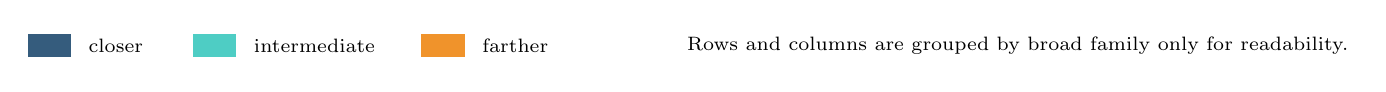
\begin{tikzpicture}[x=1cm,y=0.28cm]
\fill[UrielClose] (0,0) rectangle (0.55,1);\node[anchor=west,font=\scriptsize] at (0.65,0.5) {closer};
\fill[UrielMiddle] (2.1,0) rectangle (2.65,1);\node[anchor=west,font=\scriptsize] at (2.75,0.5) {intermediate};
\fill[UrielFar] (5.0,0) rectangle (5.55,1);\node[anchor=west,font=\scriptsize] at (5.65,0.5) {farther};
\node[anchor=west,font=\scriptsize] at (8.25,0.5) {Rows and columns are grouped by broad family only for readability.};
\end{tikzpicture}
\par\fonte{Prepared by the author (2026), based on URIEL+ featural angular distances from \textcite{khan-etal-2025-uriel}.}
\endgroup
\end{table}
\end{landscape}
}

\newcommand{\UrielLanguageMapFigure}{%
\begin{figure}[htbp]
\centering
\caption[Two-dimensional URIEL+ language-proximity map]{Classical multidimensional scaling (MDS) of the URIEL+ featural distance matrix \cite{gower1966distance}. Languages are colored by broad family.}

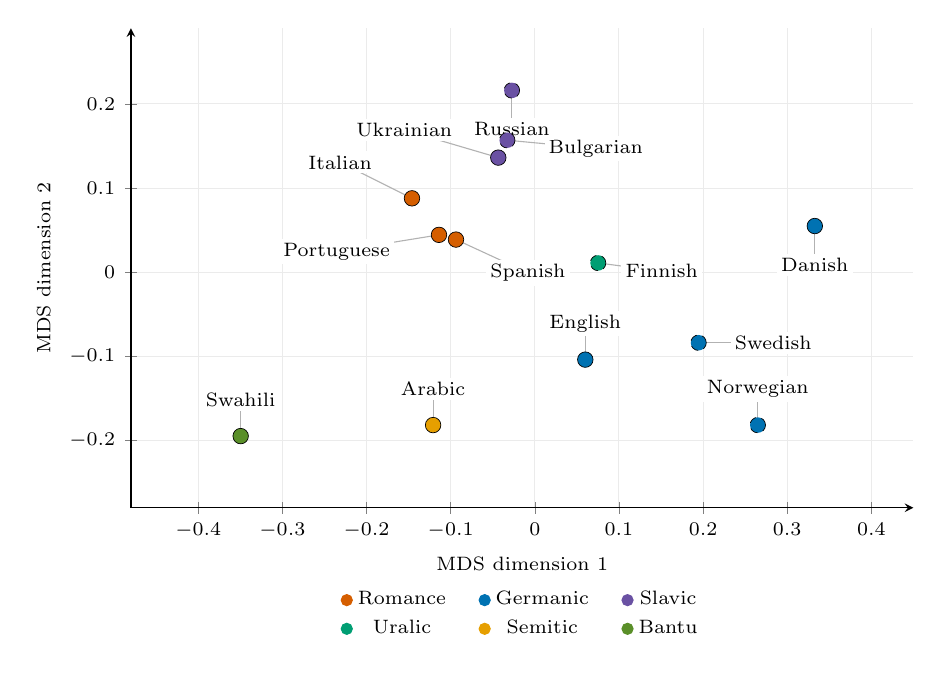
\begin{tikzpicture}
\begin{axis}[
width=0.95\linewidth,height=8.2cm,
axis lines=left,axis equal image,
xlabel={MDS dimension 1},ylabel={MDS dimension 2},
xmin=-0.48,xmax=0.45,ymin=-0.28,ymax=0.29,
grid=major,grid style={black!8},
tick label style={font=\scriptsize},
label style={font=\scriptsize},
legend columns=3,
legend style={font=\scriptsize,draw=none,fill=none,at={(0.5,-0.15)},anchor=north,
/tikz/every even column/.append style={column sep=0.35cm}},
]
\addlegendimage{only marks,mark=*,mark options={fill=UrielRomance,draw=UrielRomance}}
\addlegendentry{Romance}
\addlegendimage{only marks,mark=*,mark options={fill=UrielGermanic,draw=UrielGermanic}}
\addlegendentry{Germanic}
\addlegendimage{only marks,mark=*,mark options={fill=UrielSlavic,draw=UrielSlavic}}
\addlegendentry{Slavic}
\addlegendimage{only marks,mark=*,mark options={fill=UrielUralic,draw=UrielUralic}}
\addlegendentry{Uralic}
\addlegendimage{only marks,mark=*,mark options={fill=UrielSemitic,draw=UrielSemitic}}
\addlegendentry{Semitic}
\addlegendimage{only marks,mark=*,mark options={fill=UrielBantu,draw=UrielBantu}}
\addlegendentry{Bantu}
\addplot+[only marks,mark=*,mark size=2.8pt,mark options={fill=UrielRomance,draw=black,line width=0.25pt}] coordinates {(-0.1460,0.0878)};
\draw[black!30,thin] (axis cs:-0.1460,0.0878) -- ([xshift=-26pt,yshift=13pt]axis cs:-0.1460,0.0878);\node[font=\scriptsize,fill=white,inner sep=1.5pt,anchor=center] at ([xshift=-26pt,yshift=13pt]axis cs:-0.1460,0.0878) {Italian};
\addplot+[only marks,mark=*,mark size=2.8pt,mark options={fill=UrielRomance,draw=black,line width=0.25pt}] coordinates {(-0.1139,0.0444)};
\draw[black!30,thin] (axis cs:-0.1139,0.0444) -- ([xshift=-37pt,yshift=-6pt]axis cs:-0.1139,0.0444);\node[font=\scriptsize,fill=white,inner sep=1.5pt,anchor=center] at ([xshift=-37pt,yshift=-6pt]axis cs:-0.1139,0.0444) {Portuguese};
\addplot+[only marks,mark=*,mark size=2.8pt,mark options={fill=UrielRomance,draw=black,line width=0.25pt}] coordinates {(-0.0937,0.0388)};
\draw[black!30,thin] (axis cs:-0.0937,0.0388) -- ([xshift=26pt,yshift=-12pt]axis cs:-0.0937,0.0388);\node[font=\scriptsize,fill=white,inner sep=1.5pt,anchor=center] at ([xshift=26pt,yshift=-12pt]axis cs:-0.0937,0.0388) {Spanish};
\addplot+[only marks,mark=*,mark size=2.8pt,mark options={fill=UrielGermanic,draw=black,line width=0.25pt}] coordinates {(0.0600,-0.1039)};
\draw[black!30,thin] (axis cs:0.0600,-0.1039) -- ([xshift=0pt,yshift=13pt]axis cs:0.0600,-0.1039);\node[font=\scriptsize,fill=white,inner sep=1.5pt,anchor=center] at ([xshift=0pt,yshift=13pt]axis cs:0.0600,-0.1039) {English};
\addplot+[only marks,mark=*,mark size=2.8pt,mark options={fill=UrielGermanic,draw=black,line width=0.25pt}] coordinates {(0.3328,0.0549)};
\draw[black!30,thin] (axis cs:0.3328,0.0549) -- ([xshift=0pt,yshift=-14pt]axis cs:0.3328,0.0549);\node[font=\scriptsize,fill=white,inner sep=1.5pt,anchor=center] at ([xshift=0pt,yshift=-14pt]axis cs:0.3328,0.0549) {Danish};
\addplot+[only marks,mark=*,mark size=2.8pt,mark options={fill=UrielGermanic,draw=black,line width=0.25pt}] coordinates {(0.2650,-0.1817)};
\draw[black!30,thin] (axis cs:0.2650,-0.1817) -- ([xshift=0pt,yshift=13pt]axis cs:0.2650,-0.1817);\node[font=\scriptsize,fill=white,inner sep=1.5pt,anchor=center] at ([xshift=0pt,yshift=13pt]axis cs:0.2650,-0.1817) {Norwegian};
\addplot+[only marks,mark=*,mark size=2.8pt,mark options={fill=UrielGermanic,draw=black,line width=0.25pt}] coordinates {(0.1946,-0.0838)};
\draw[black!30,thin] (axis cs:0.1946,-0.0838) -- ([xshift=27pt,yshift=0pt]axis cs:0.1946,-0.0838);\node[font=\scriptsize,fill=white,inner sep=1.5pt,anchor=center] at ([xshift=27pt,yshift=0pt]axis cs:0.1946,-0.0838) {Swedish};
\addplot+[only marks,mark=*,mark size=2.8pt,mark options={fill=UrielUralic,draw=black,line width=0.25pt}] coordinates {(0.0752,0.0110)};
\draw[black!30,thin] (axis cs:0.0752,0.0110) -- ([xshift=23pt,yshift=-3pt]axis cs:0.0752,0.0110);\node[font=\scriptsize,fill=white,inner sep=1.5pt,anchor=center] at ([xshift=23pt,yshift=-3pt]axis cs:0.0752,0.0110) {Finnish};
\addplot+[only marks,mark=*,mark size=2.8pt,mark options={fill=UrielSlavic,draw=black,line width=0.25pt}] coordinates {(-0.0328,0.1569)};
\draw[black!30,thin] (axis cs:-0.0328,0.1569) -- ([xshift=32pt,yshift=-3pt]axis cs:-0.0328,0.1569);\node[font=\scriptsize,fill=white,inner sep=1.5pt,anchor=center] at ([xshift=32pt,yshift=-3pt]axis cs:-0.0328,0.1569) {Bulgarian};
\addplot+[only marks,mark=*,mark size=2.8pt,mark options={fill=UrielSlavic,draw=black,line width=0.25pt}] coordinates {(-0.0273,0.2161)};
\draw[black!30,thin] (axis cs:-0.0273,0.2161) -- ([xshift=0pt,yshift=-14pt]axis cs:-0.0273,0.2161);\node[font=\scriptsize,fill=white,inner sep=1.5pt,anchor=center] at ([xshift=0pt,yshift=-14pt]axis cs:-0.0273,0.2161) {Russian};
\addplot+[only marks,mark=*,mark size=2.8pt,mark options={fill=UrielSlavic,draw=black,line width=0.25pt}] coordinates {(-0.0434,0.1362)};
\draw[black!30,thin] (axis cs:-0.0434,0.1362) -- ([xshift=-34pt,yshift=10pt]axis cs:-0.0434,0.1362);\node[font=\scriptsize,fill=white,inner sep=1.5pt,anchor=center] at ([xshift=-34pt,yshift=10pt]axis cs:-0.0434,0.1362) {Ukrainian};
\addplot+[only marks,mark=*,mark size=2.8pt,mark options={fill=UrielSemitic,draw=black,line width=0.25pt}] coordinates {(-0.1209,-0.1817)};
\draw[black!30,thin] (axis cs:-0.1209,-0.1817) -- ([xshift=0pt,yshift=13pt]axis cs:-0.1209,-0.1817);\node[font=\scriptsize,fill=white,inner sep=1.5pt,anchor=center] at ([xshift=0pt,yshift=13pt]axis cs:-0.1209,-0.1817) {Arabic};
\addplot+[only marks,mark=*,mark size=2.8pt,mark options={fill=UrielBantu,draw=black,line width=0.25pt}] coordinates {(-0.3496,-0.1948)};
\draw[black!30,thin] (axis cs:-0.3496,-0.1948) -- ([xshift=0pt,yshift=13pt]axis cs:-0.3496,-0.1948);\node[font=\scriptsize,fill=white,inner sep=1.5pt,anchor=center] at ([xshift=0pt,yshift=13pt]axis cs:-0.3496,-0.1948) {Swahili};
\end{axis}
\end{tikzpicture}

\label{fig:uriel-language-map}
\fonte{Prepared by the author (2026), based on URIEL+ featural angular distances from \textcite{khan-etal-2025-uriel}.}
\end{figure}
}

\newcommand{\AttackLanguageSpeakerMapFigure}{%
\begin{figure}[htbp]\centering
\caption[Attack-language speaker map]{Representative speaker communities for the thirteen attack languages, with a European inset. Transnational languages appear at multiple locations; color identifies the language and marker size encodes its total-speaker bin.}

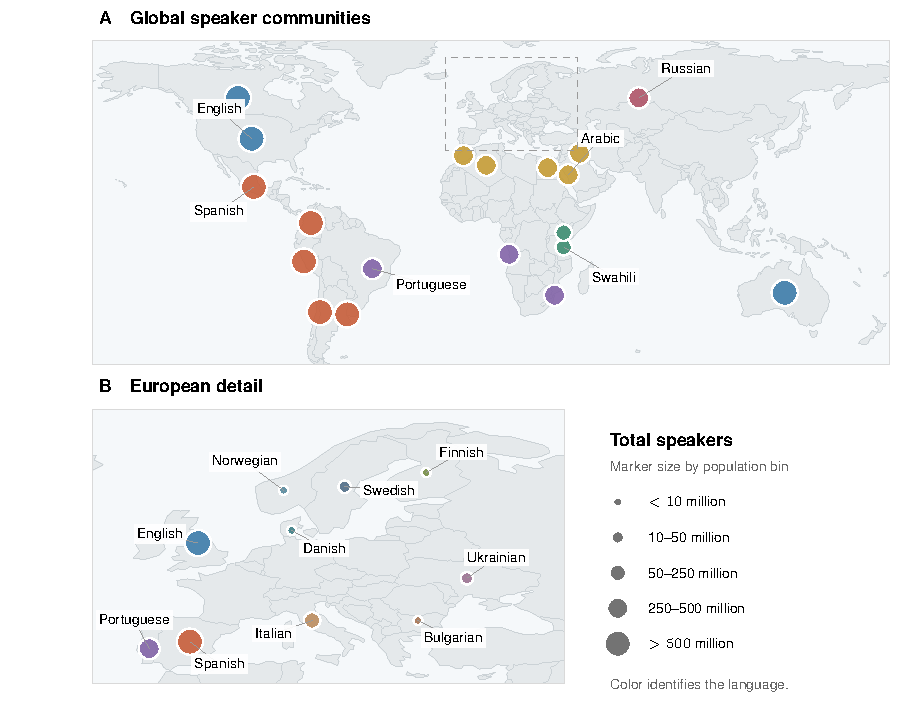
\includegraphics[max width=\linewidth]{figures/compiled/attack_language_map.pdf}

\label{fig:attack-language-speaker-map}
\fonte{Prepared by the author (2026), based on Natural Earth country boundaries and speaker estimates from \textcite{eberhard2025ethnologue}; reference locations informed by \textcite{hammarstrom2026glottolog}.}
\end{figure}}

